% ============================================================
% 1C
% ============================================================

\section{Task 1C: SIMD}

\subsection{Baseline Instruction Count}
For a $512 \times 512$ matrix with a kernel size of $K=5$, the naive baseline implementation executed $\sim$1.31 billion instructions.

\subsection{SIMD Implementations}
The convolution algorithm was parallelized using Intel AVX intrinsics . The inner spatial loop was stepped by the SIMD vector width (e.g., 8 floats for 256-bit AVX2) . Both 128-bit (SSE) and 256-bit (AVX2) implementations were evaluated across different matrix sizes to measure vectorization efficiency.

\begin{table}[H]
\centering
\caption{Task 1C SIMD results ($K=5$)}
\begin{tabular}{lcccc}
\toprule
Matrix Size & SIMD Width & Instructions & Time (ms) & Speedup \\
\midrule
$512 \times 512$   & 128-bit & 296,643,371   & 0.466 & 8.40$\times$ \\
$512 \times 512$   & 256-bit & 158,009,805   & 0.522 & 7.95$\times$ \\
$1024 \times 1024$ & 128-bit & 1,183,171,431 & 2.175 & 7.10$\times$ \\
$1024 \times 1024$ & 256-bit & 628,631,602   & 2.189 & 7.74$\times$ \\
$2048 \times 2048$ & 256-bit & 2,510,515,355 & 9.150 & 7.47$\times$ \\
\bottomrule
\end{tabular}
\end{table}

\subsection{SIMD Intrinsics}

\begin{itemize}
    \item \texttt{\_mm256\_setzero\_ps}: Purpose: Initializes a 256-bit accumulator vector to zero . Justification: Needed to clear the parallel accumulator state before summing the kernel convolution .
    \item \texttt{\_mm256\_loadu\_ps} / \texttt{\_mm256\_storeu\_ps}: Purpose: Loads/stores 8 contiguous floats to/from memory. Unaligned loads and stores were used because 32-byte alignment cannot be guaranteed for every accessed address.
    \item \texttt{\_mm256\_set1\_ps}: Purpose: Broadcasts a single kernel weight into all 8 lanes of the SIMD register . Justification: During a single kernel step, the same weight must be multiplied simultaneously against 8 adjacent spatial input pixels .
    \item \texttt{\_mm256\_fmadd\_ps}: Purpose: Fused multiply-add. It performs the multiply-add in one fused vector instruction, reducing instruction count and improving arithmetic throughput.
\end{itemize}

\subsection{Speedup Plots}

\begin{figure}[H]
    \centering
    \begin{subfigure}{0.48\textwidth}
        \centering
        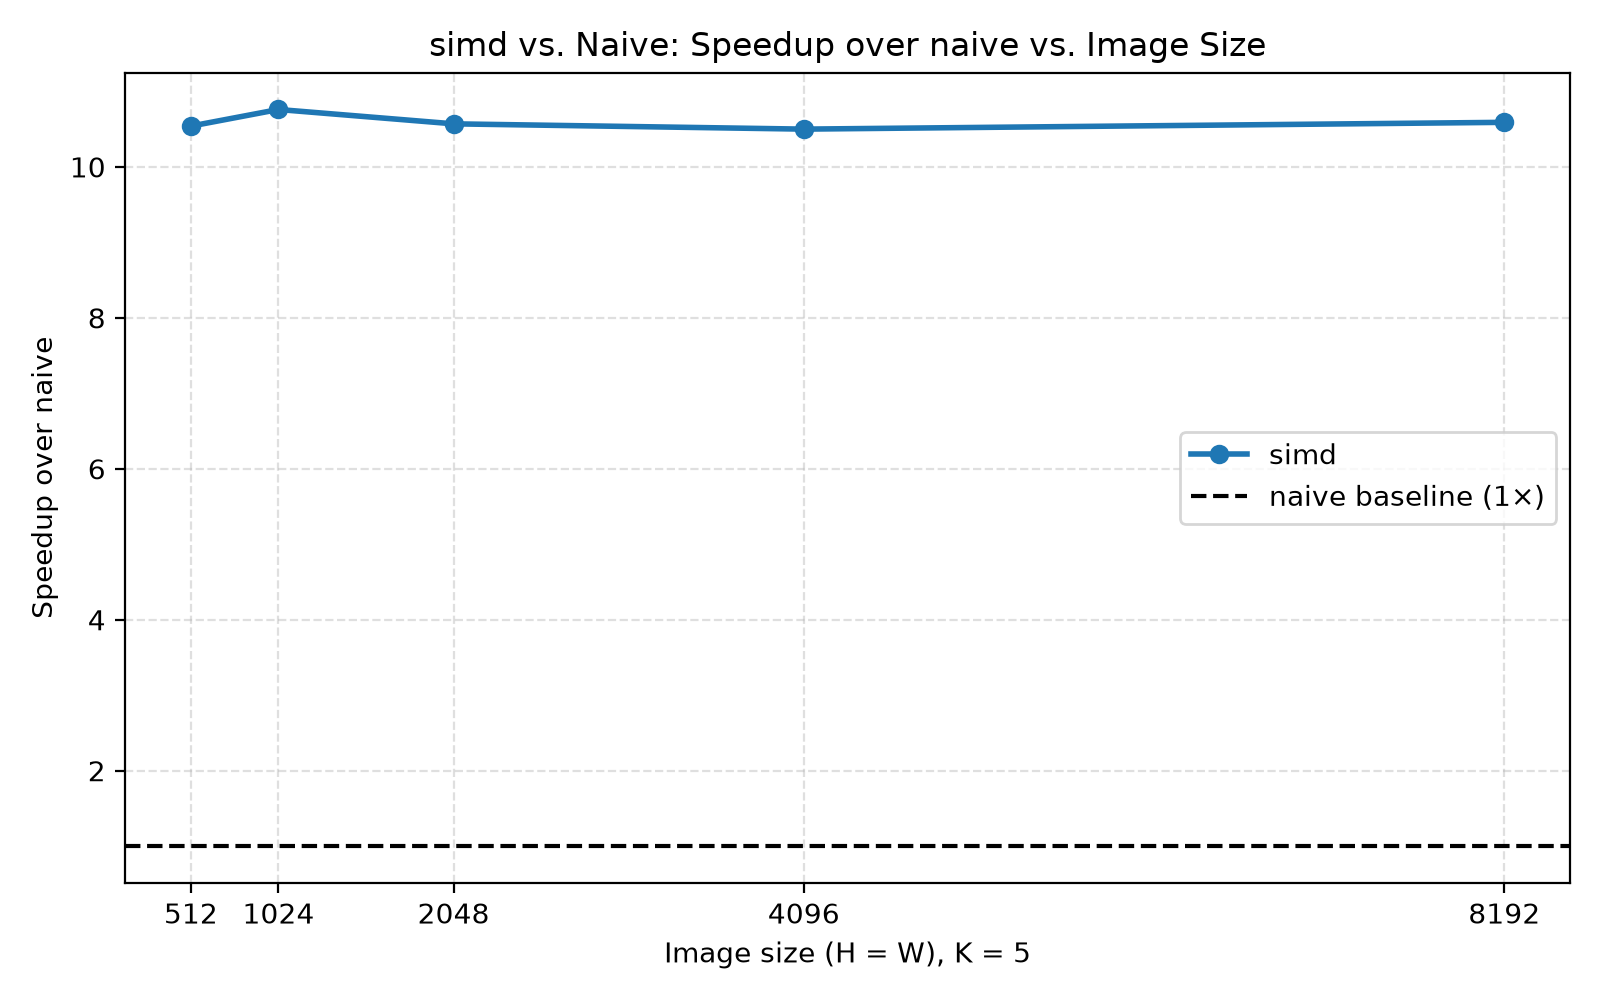
\includegraphics[width=\linewidth]{plots/task1c/simd_vs_naive_speedup_image_size_k5.png}
        \caption{Speedup vs. Image Size ($K=5$)}
    \end{subfigure}
    \hfill
    \begin{subfigure}{0.48\textwidth}
        \centering
        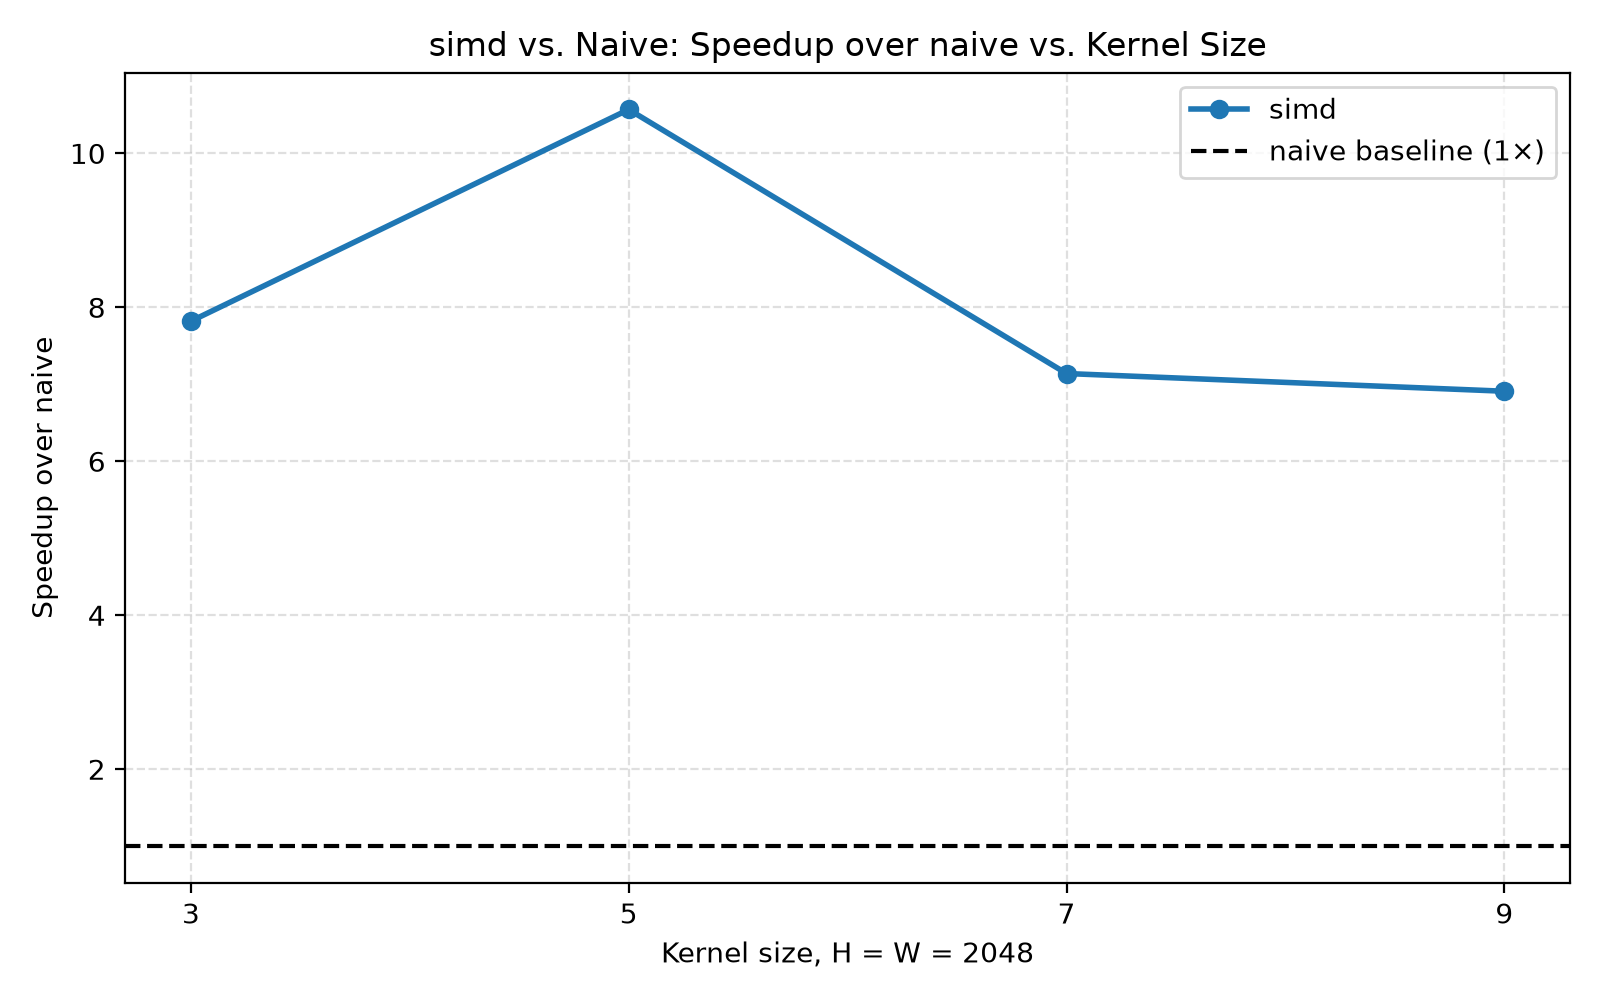
\includegraphics[width=\linewidth]{plots/task1c/simd_vs_naive_speedup_kernel_size_2048.png}
        \caption{Speedup vs. Kernel Size ($2048 \times 2048$)}
    \end{subfigure}
    
    \vspace{1em}
    \begin{subfigure}{0.48\textwidth}
        \centering
        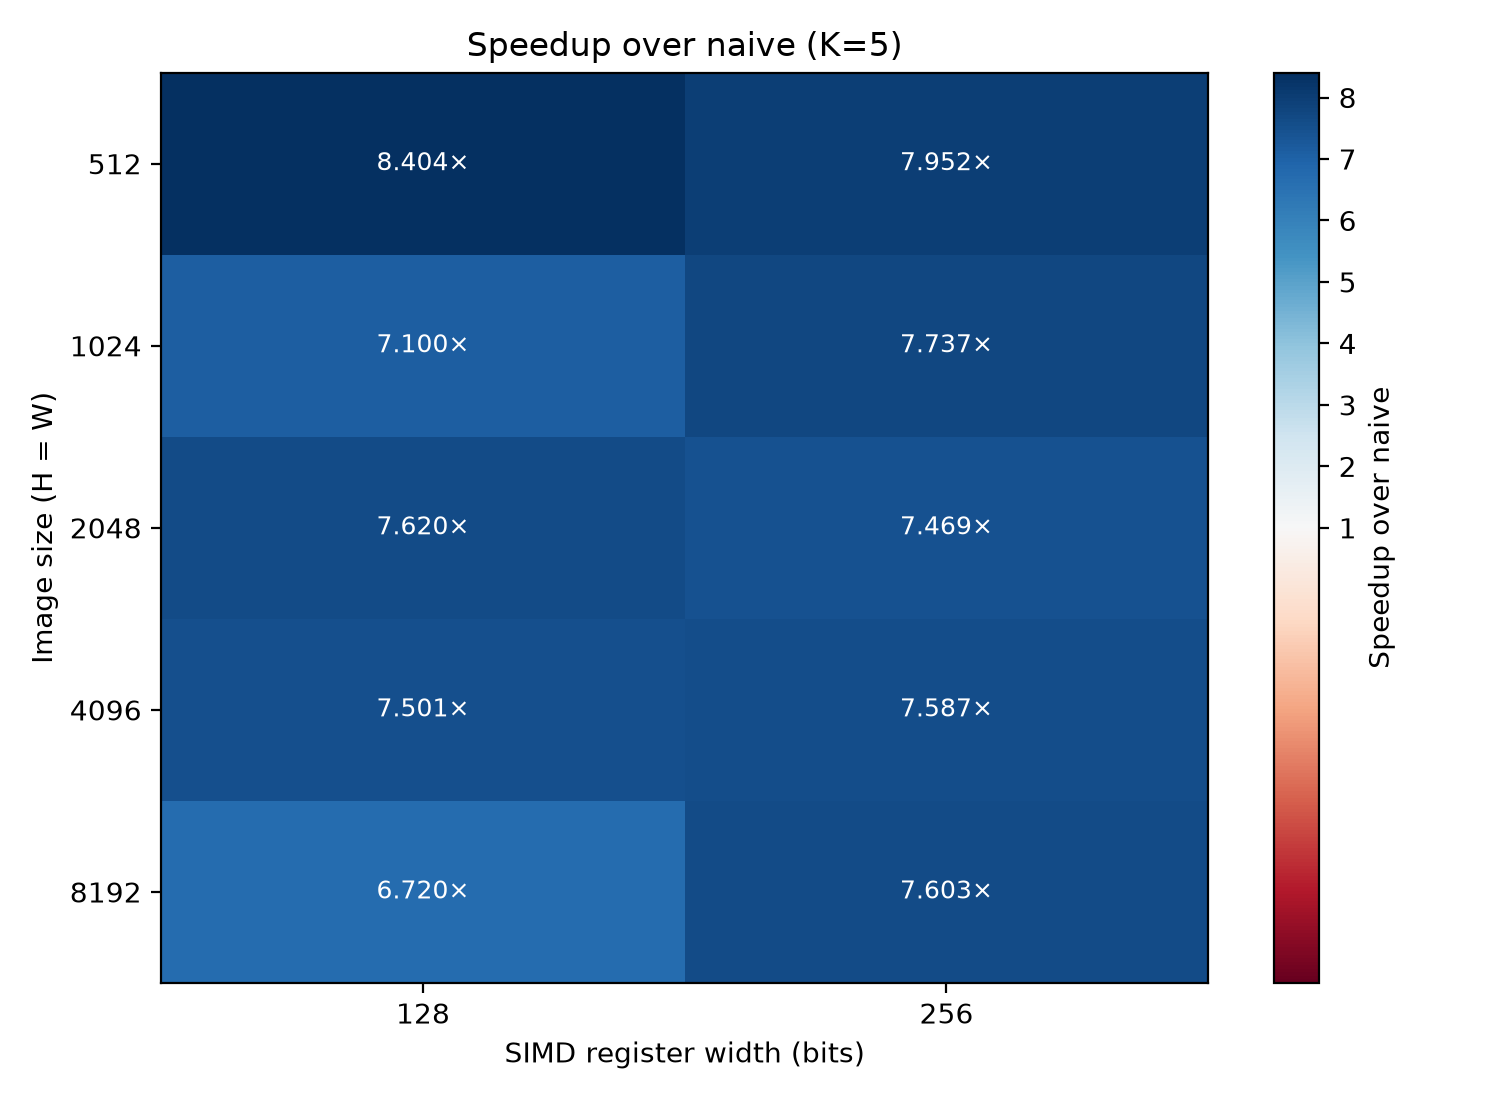
\includegraphics[width=\linewidth]{plots/task1c/speedup_heatmap_k5.png}
        \caption{Speedup Heatmap (Width vs Image Size)}
    \end{subfigure}
    \hfill
    \begin{subfigure}{0.48\textwidth}
        \centering
        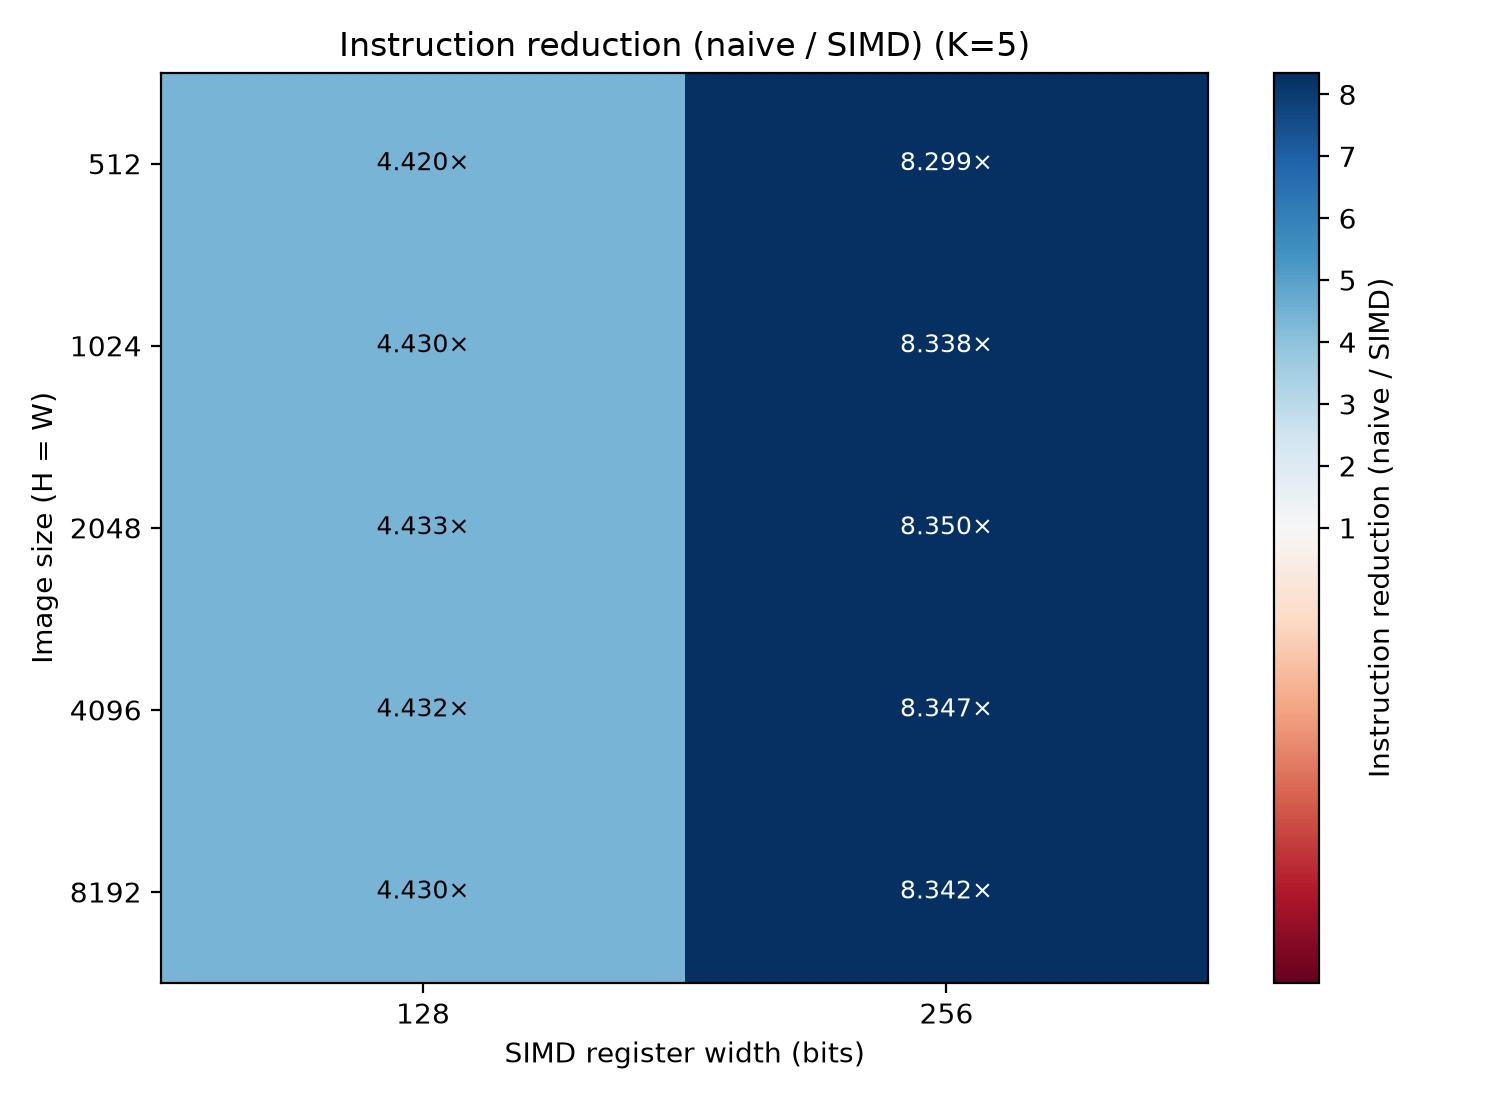
\includegraphics[width=\linewidth]{plots/task1c/instruction_reduction_heatmap_k5.png}
        \caption{Instruction Reduction Factor}
    \end{subfigure}
    \caption{SIMD performance and hardware metric improvements.}
\end{figure}

\subsection{Analysis}
SIMD substantially reduced the executed instruction count. A 128-bit vector instruction processes 4 single-precision values, while a 256-bit AVX2 vector instruction processes 8. The measured instruction reductions were approximately $4.4\times$ and $8.3\times$, respectively; realized performance also depends on loads, scheduling, and reduction overhead.

Interestingly, while 256-bit SIMD approximately halved the instructions compared to 128-bit, the raw speedup did not double. At a $1024 \times 1024$ image size, 256-bit offered a marginal speedup advantage over 128-bit ($7.74\times$ vs $7.10\times$). This indicates that data-delivery throughput and other memory-system effects become more important than arithmetic instruction count alone. Bandwidth and cache latency are distinct effects, and these measurements do not isolate either one.

\subsection{Questions}

\begin{enumerate}
    \item \textbf{How did the instruction count change?} \\
    The instruction count fell by $\sim$4.4 for the 128-bit version and $\sim$8.3 for the 256-bit version compared with the naive baseline. These reductions are consistent with processing 4 and 8 floats per vector instruction, respectively.
    \item \textbf{Did you achieve speedup? Why?} \\
    Yes, speedups of roughly $7\times$ to $8\times$ were observed. Data parallelism, fused vector multiply-add instructions, and lower loop-control overhead all contributed; the vector width specifies elements per instruction, not a guaranteed number of elements per cycle.
    \item \textbf{Which SIMD intrinsics were used and why?} \\
    We primarily used \texttt{\_mm256\_loadu\_ps} for safe unaligned memory reads, \texttt{\_mm256\_set1\_ps} to broadcast scalar weights to all vector lanes, and \texttt{\_mm256\_fmadd\_ps} for the core fused accumulation. The unaligned operations avoid requiring every sliding-window address to be 32-byte aligned.
\end{enumerate}
